\documentclass[12pt,a4paper,twocolumn]{article}
\usepackage{preamble} % all preamble code is located in preamble.sty

\begin{document}
\pagenumbering{gobble}  

\includepdf[]{assets/cover.pdf} 

\newpage

\title{Rover Technical Documentation}
\author{AU-Robotics}

\renewcommand{\contentsname}{}



\newcommand{\university}{\textbf{Alexandria University\\Faculty of Engineering}}
\newcommand{\teamname}{\textbf{Alexandria University Robotics}}
\newcommand{\vehiclename}{\textbf{Rover Name: Phoenix}}
\newcommand{\leadername}{\textbf{Team Leader: Youssef Samy}}
\newcommand{\email}{\textbf{Email: office.youssefkassem@gmail.com }}

\begin{titlepage}
    \centering
    {\LARGE \university \par}
    \vspace{0.3cm}
    
    {\Large \teamname \par}
    \vspace{0.1cm}
    
    {\Large \vehiclename \par}
    \vspace{0.3cm}
    
    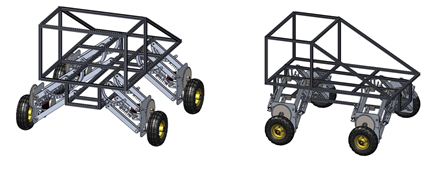
\includegraphics[width=0.7\textwidth]{assets/rover.png} 
        \vspace{-0.5cm}

    {\large \leadername \par}
    {\large \email \par}
    % \vfill
    {\large \today \par}
\section*{Contents}
\begin{multicols}{2}
    \tableofcontents
\end{multicols}

\end{titlepage}

\newpage
\pagenumbering{arabic}   % Restart page numbers
\setcounter{page}{1}     % Explicitly set page number to 1
\section{Introduction}

\subsection{Overview}

Founded by a group of engineering students at Alexandria University, our team was formed with the vision of applying theoretical knowledge to real-world robotics challenges through a collaborative, hands-on approach.

We are proudly participating in the \textbf{International Competition of the Military Technical College: Unmanned Ground Vehicle Challenge of 2026 (UGVC)}.
We aim to strengthen our experience with reliable rover technologies and produce a better performing rover compared to our attempt last year.

\subsection{Team Organization}

Our team is organized into four core technical departments: \textbf{Software}, \textbf{Firmware}, \textbf{Hardware}, and \textbf{Mechanical}.
Each department is led by a Head and supported by a Vice Head and a dedicated team of engineers. This structure ensures clear task distribution, streamlined communication, and high-performance coordination across disciplines.

\textbf{Executive Board:}
\begin{itemize}
    \setlength{\itemsep}{1pt}
    \setlength{\parskip}{0pt}
    \setlength{\parsep}{0pt}
    \item \textbf{Habiba Abdulhameed} -- Supervisor \& COO
    \item \textbf{Ahmad Zaki} (4th Year) -- CEO
    \item \textbf{Youssef Samy} (3rd Year) -- CTO
    \item \textbf{Shahd Yasser} (4th Year) -- CFO
\end{itemize}

\textbf{Software Team:}
\begin{itemize}
    \setlength{\itemsep}{1pt}
    \setlength{\parskip}{0pt}
    \setlength{\parsep}{0pt}
    \item \textbf{Head:} Abdelaziz Islam (3rd Year)
    \item \textbf{Vice Head:} Mohamed ElTahhan (3rd Year)
    \item \textbf{Team Members:}
    \begin{itemize}
        \setlength{\itemsep}{1pt}
        \setlength{\parskip}{0pt}
        \setlength{\parsep}{0pt}
        \item Yahya Hussein (2nd Year)
        \item Yassin Awad (2nd Year)
        \item Nada Osama (2nd Year)
        \item Yassin Salhin (3rd Year)
        \item Yassin Ezzat (4th Year)
        \item Mohab Tantawy (3rd Year)
    \end{itemize}
\end{itemize}

\textbf{Firmware Team:}
\begin{itemize}
    \setlength{\itemsep}{1pt}
    \setlength{\parskip}{0pt}
    \setlength{\parsep}{0pt}
    \item \textbf{Head:} Ahmed Motawe (3rd Year)
    \item \textbf{Vice Head:} Rowan Mokhtar (4th Year)
    \item \textbf{Team Members:}
    \begin{itemize}
        \setlength{\itemsep}{1pt}
        \setlength{\parskip}{0pt}
        \setlength{\parsep}{0pt}
        \item Ahmed Elmasry (3rd Year)
        \item Youssra Farghaly (2nd Year)
        \item Dania Ahmed (4th Year)
        \item Abdulrahman Khaled (2nd Year)
        \item Zeyad Ayman (3rd Year)
        \item Abdullah Kassem (2nd Year)
    \end{itemize}
\end{itemize}

\textbf{Hardware Team:}
\begin{itemize}
    \setlength{\itemsep}{1pt}
    \setlength{\parskip}{0pt}
    \setlength{\parsep}{0pt}
    \item \textbf{Head:} Asser Maged (3rd Year)
    \item \textbf{Vice Head:} Youssef Nasser (2nd Year)
\end{itemize}

\textbf{Mechanical Team:}
\begin{itemize}
\setlength{\itemsep}{1pt}
    \setlength{\parskip}{0pt}
    \setlength{\parsep}{0pt}
    \item \textbf{Head:} Khaled Gado (4th Year)
    \item \textbf{Team Members:}
    \begin{itemize}
    \setlength{\itemsep}{1pt}
    \setlength{\parskip}{0pt}
    \setlength{\parsep}{0pt}
        \item Seif ul Islam (4th Year)
        \item Mohamed Hawash (3rd Year)
    \end{itemize}
\end{itemize}

\section{Design Process}

\subsection{Requirement Definition}

Aided by our prior experience and knowledge of constraints, it was identified that the design must:

\begin{itemize}
    \setlength{\itemsep}{1.2pt}
    \setlength{\parskip}{0pt}
    \setlength{\parsep}{0pt}
    \item Withstand impacts from rocky and sandy terrain
    \item Maintain traction and stability during sharp turns
    \item Be manufacturable using accessible local resources
    \item Have zero-error emergency access mechanisms
    \item Have responsive navigation via performant compute
\end{itemize}

\subsection{Software Tools}

The rover's design and development followed an iterative, modular, prototype-aided, test-driven approach.
The following software suite that allowed testing, simulation, design and telemetry plotting was used:

\begin{itemize}
    \setlength{\itemsep}{1pt}
    \setlength{\parskip}{0pt}
    \setlength{\parsep}{0pt}
    \item \textbf{Gazebo + RViz:} For simulating sensors, testing navigation, and visual debugging
    \item \textbf{MATLAB + Simulink:} For control system design, PID tuning, and motor modeling using the System Identification Toolbox
    \item \textbf{OpenCV + YOLO:} For all computer vision-based modules including lane, obstacle, and pothole detection
    \item \textbf{Git Monorepo:} For collaborative version control and agile task tracking
    \item \textbf{Docker \& Pixi:} Used to standardize development environments across the software team
    \item \textbf{Python (pySerial, adbutils, Qt6):} For serial communication, sensor parsing, and real-time plotting during testing
    \item \textbf{Custom Embedded Debugger:} For interactive ROS $\leftrightarrow$ MCU communication over UART.
\end{itemize}

This toolset enabled parallel development across subsystems, with 

\subsection{Budget Management}
Phoenix was designed within a tightly constrained budget. Chosen components had to be reliable in a cost-effective way. Our budgeting practices included:

\begin{itemize}
    \item \textbf{Modular PCBs:} Separated logic, power, and motor
    boards for reusability and easier debugging
    \item \textbf{Software Spending:} Leveraged ROS 2, Gazebo, OpenCV, along with MATLAB and Solidworks with student licenses
    \item \textbf{Component prioritization:} Focused spending on mission-critical components like IMU (\texttt{BNO055}), GPS (\texttt{NEO-6M}), and motor encoders
    \item \textbf{Efficient power delivery:} Dual battery packs (2x12V in series) with DC-DC buck converters ensured safe power distribution without needing expensive power modules
    \item \textbf{Local sourcing \& salvaging:} Some structural and passive components were recycled from past projects or obtained from local vendors at reduced cost
    \item \textbf{Contingency Planning:} $\approx 10\%$ of the budget was reserved for hardware replacements due to risk of burnouts during testing
\end{itemize}

All financials and payments were tracked using shared spreadsheets with saved history for tracking iterations and pricing fluctuations.

\subsection{Safety Measures}

Safety was a core design consideration both in hardware and software.
\paragraph{Hardware Safety:}


\paragraph{Software Safety:}

\section{Technical Innovation}

\subsection{Mechanical Innovations}

\subsection{Software Innovations}

\section{Mechanical Design}
\subsection{Design Improvement}
\subsection{Frame Design}
\subsection{Laser Pointer}
\subsection{Hardware Box}

\section{Electronic and Power Design}
\subsection{Main Control Unit}
\subsection{Motor Control Board}
\subsection{Power Board}

\section{Software Design}

\subsection{System Architecture Overview}
\subsection{Core Functionalities}
\subsubsection{Lane Detection and Navigation}
% lane detection part
% lane navigation part 
The rover's lateral offset from the lane center, output by the \texttt{lane\_detection\_node}, is consumed by the lane navigation module as its error input. Lane navigation is handled by a PID control loop that converts this error into a corrective angular velocity command, while maintaining a constant forward velocity.
\\
The PID controller is tuned to provide a balance between responsiveness and stability in MATLAB's Simulink as shown in Figure \ref{fig:pid-tuning}.
\begin{figure}[H]
    \centering
    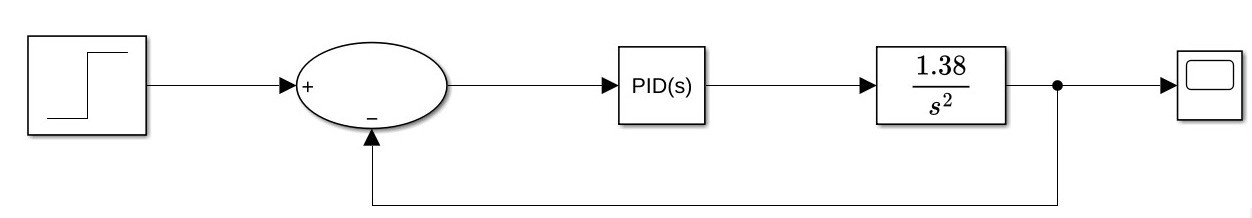
\includegraphics[width=0.75\linewidth]{assets/lane_control_loop.jpeg}
    \caption{PID Tuning }
    \label{fig:pid-tuning}
\end{figure}
\begin{figure}[H]
    \centering
    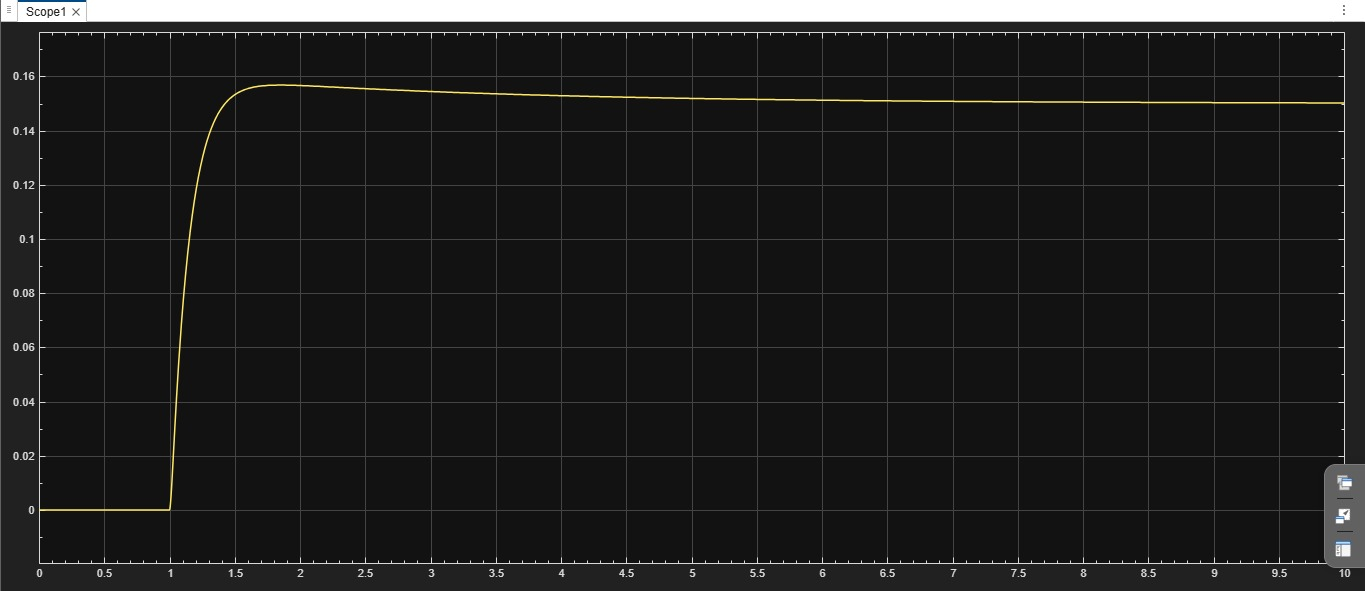
\includegraphics[width=0.75\linewidth]{assets/lane_control_response.jpeg}
    \caption{PID step response for lane navigation control}
    \label{fig:lane-control-response}
\end{figure}
\textbf{Safety and Stability Considerations:} 
\begin{itemize}
    \setlength{\itemsep}{1pt}
    \setlength{\parskip}{0pt}
    \setlength{\parsep}{0pt}
    \item Integral windup protection: The accumulated integral term is bounded to ±1.0, preventing the integral component from growing unbounded during sustained non-zero error.
    \item Angular velocity saturation:  The final steering command is clamped to a max angular velocity, ensuring the rover cannot issue a steering command beyond necessary limits.
\end{itemize}
The lane navigation node then publishes the steering commands to the respective topic to be processed along with the obstacle avoidance node's output to generate a final angular velocity command for the rover.

\subsubsection{Pothole Detection}
\subsubsection{Obstacle Avoidance}
The rover utilizes a LiDAR sensor (RPLIDAR A2)  to detect obstacles within the drivable lane corridor and generate a corrected heading that keeps the rover within lane boundaries while avoiding collisions.
The algorithm is a modified version of the \textbf{Disparity Extender} technique,constrained to an angular Region of Interest (ROI) aligned with the rover's current lane heading, rather than considering the entire 360-degree scan.
This design ensures that the obstacle avoidance is treated as a local heading correction relative to the lane-following reference, preveting the rover from selecting a safe gap that would take it outside the lane.
\begin{figure}[H]
    
    \centering
    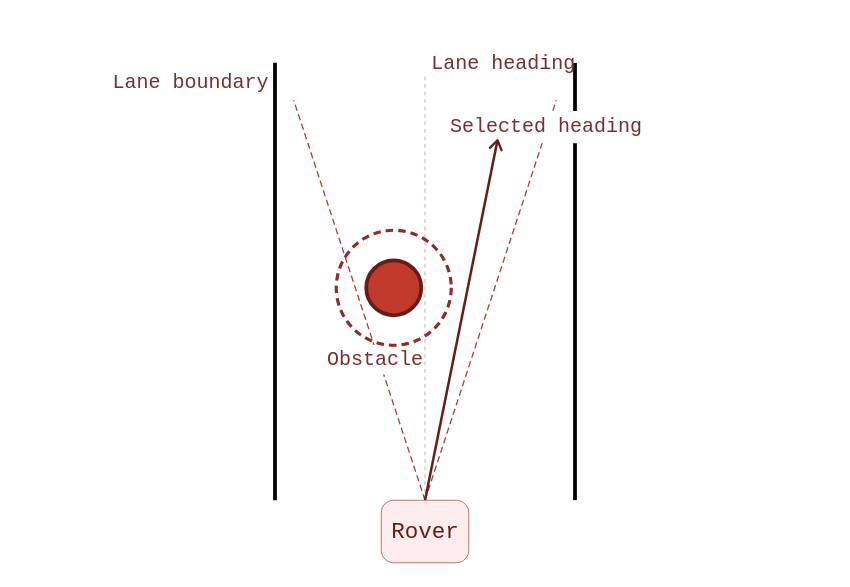
\includegraphics[width=0.75\linewidth]{assets/lidar_avoid.png}
    \caption{Obstacle Avoidance Algorithm}
    \label{fig:obstacle-avoidance}
\end{figure}

At each scan cycle, the system executes the following sequence:
\begin{enumerate}
    \setlength{\itemsep}{1pt}
    \setlength{\parskip}{0pt}
    \setlength{\parsep}{0pt}
    \item \textbf{Scan Acquisition:} The LiDAR provides distance readings across its full field of view.
    \item \textbf{Region of Interest Restriction:} The system receives the lane information and limits further processing to a defined angular window around that heading.
    \item \textbf{Obstacle Edge Detection:} Within this window, the system identifies significant discontinuities between adjacent distance readings. These discontinuities indicate the physical edges of obstacles
    \item \textbf{Boundary Expansion:} Each detected obstacle edge is extended outward by a distance corresponding to the rover's physical width plus an additional safety margin. This prevents the selection of a path that appears clear but would be insufficient for the rover to pass through safely.
    \item \textbf{Heading Selection:} Following boundary expansion, select the direction within the permitted window that offers the greatest unobstructed distance and publish this as the corrected heading command.
\end{enumerate}


\subsubsection{Face Recognition and Detection}
\paragraph{Models:}
The system uses two pre-trained OpenCV deep learning models. YuNet is used for real-time face detection, while SFace extracts facial features and performs face recognition by comparing the detected face with a stored target feature using cosine similarity. The target feature is cached after the first extraction to improve runtime performance.

\paragraph{Architecture:}
The system implements a real-time face recognition pipeline that processes live camera frames. It first detects faces in each frame, then recognizes the target person by comparing the detected face with a stored facial representation. The output indicates whether the detected face matches the target or is an unknown person.

For a recognized target, the system also estimates the face position relative to the center of the image by computing horizontal and vertical offsets. This information can be used for real-time tracking or robot navigation while continuously updating the visual output.

\begin{figure}[H]
    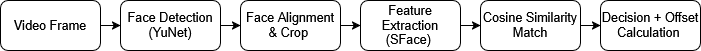
\includegraphics[width=0.45\textwidth]{assets/Face Recognition Pipeline.png}
    \caption{Face Recognition Pipeline}
\end{figure}

\paragraph{ROS Integration:}
The face recognition node subscribes to the video stream to process each frame, and publishes the annotated frame for optional debugging along with a coordinate offset for laser pointing.

\subsection{Communication Systems}
For transfering high-speed, high-bandwidth data between the onboard computer and the station, the existing ROS 2 system with its Data Distribution Service was used, to leverage descriptive topics, concurrent querying, real-time streaming and fault-tolerant connection.

For station-rover communication, the onboard computer has an exposed 6 dBi unidirectional antenna, which is connected via a USB-A adapter directly to a PCIe bus rather than the shared USB bus for cameras to prevent internal bus congestion.
By tuning the QoS profile for each telemetry topic, high-throughput non-critical streams like the camera streams have a reduced error-recovery load on the DDS.
The station's router is configured to have a narrower wireless bandwidth (5-20 MHz) and shortened range (250m) for a robust, focused signal.

\subsection{Auxiliary Systems}
\subsubsection{Motor Control}
\subsubsection{Sensor Fusion}
\subsubsection{Vehicle Monitoring}
\subsection{System Integration}
\subsection{Software Testing and Bug Tracking}


\section{Future Work}

The mechanical team aims to implement:

\begin{enumerate}[label=\textbf{\alph*.}, itemsep=1pt, parsep=0pt]
    \item \textbf{Active Suspension:} Servo-controlled or fluid-based damping systems for terrain-adaptive ride quality.
    \item \textbf{Lightweighting:} FEA and topology optimization to reduce mass without sacrificing strength.
    \item \textbf{Sealed Joints:} Sand-proof bearing housings and maintenance-friendly component designs.
    \item \textbf{Integrated Drive Units:} Compact gearboxes with aligned shafts, improved torque, and shock resistance.
    \item \textbf{Adjustable Frame Geometry:} Tunable suspension height, wheelbase, and CG for better terrain adaptability.
    \item \textbf{Manufacturing:} CNC bending, jig expansion, and QA protocols for consistency and precision.
\end{enumerate}

\vspace{1em}

For electrical improvements, the team plans to:

\begin{itemize}[itemsep=1pt]
    \setlength{\parskip}{0pt}
    \setlength{\parsep}{0pt}
    \item Design custom microcontrollers tailored to system needs.
    \item Develop in-house buck converters and motor drivers.
    \item Enhance subsystem coordination and autonomy via smarter control algorithms.
\end{itemize}

These changes aim to deepen hardware understanding, boost customization, and improve adaptability for complex tasks and terrains.

\addcontentsline{toc}{section}{References}
\nocite{*}
\bibliographystyle{plain}
\small
\bibliography{references}


\end{document}